\documentclass{article}

\usepackage{url}
\usepackage{cite}
\usepackage{mhchem}
\usepackage{graphicx}
\usepackage{subfigure}
\usepackage[a4paper,top=2cm,bottom=2cm,left=3cm,right=3cm,marginparwidth=1.75cm]{geometry}

\title{SARS-CoV-2 3CL Protease Gene Cloning}
\author{Yan Haoming\\2300017744}
\date{September 13, 2024}

\begin{document}
\maketitle
\begin{abstract}
    3CL protease (3C-like protease) is the main protease found in coronavirus (SARS-CoV-2) playing an important role in the processing of coronavirus replicase polyprotein\cite{websiteKey}.
    Therefore, it is meaningful to study the 3CL protease and in this experiment we started with cloning the 3CL protease gene.
    
    The major purpose of this experiment was to construct recombinant plasmid vector for future gene expression.
    So we started from amplifying desired DNA by PCR along with DNA separation and purification by electrophoresis.
    DNA quantification was needed before assembling the plasmid by Gibson assembly.
    The final step was to transform the bacteria (\textit{E.coli} DH5$\alpha$ strain) with the plasmid vector to store and reproduce the expression vector.

    In this report, I record the experimental methods with the detailed analysis of the results so as to set the cornerstone for future experiments and scientific enquiry.
\end{abstract}
\textbf{Keywords:} SARS-CoV-2, 3CL protease, PCR, Agarose-gel Electrophoresis, Gel Extraction, Gibson Assembly, Transformation.
\section{Interpretation of the Plasmid}
    \begin{figure}
    \centering
    \includegraphics[width=0.75\linewidth]{../Figures/plasmid.png}
    \caption{Desired Recombinant Plasmid}
    \label{Desired Recombinant Plasmid}
    \end{figure}
    The components on the plasmid are important for experimental methods and processes, so I find it deserves a deeper look.
    
    As shown in Figure \ref{Desired Recombinant Plasmid}, the 3CL protease gene should be inserted between \textbf{T7 promoter and T7 terminator}.
    However, a \textbf{Lac operator}\cite{TheCell} is placed in the upstream of 3CL protease gene, while \textbf{LacI gene} expressing \textbf{Lac repressor} is also present in the plasmid, which means the expression of 3CL protease gene will be repressed.
    Indeed, we transform the bacterial strain of \textbf{DH5$\alpha$} which also lacks of \textbf{T7 polymerase}.
    That means in this step we focus on cloning the 3CL protease gene only without expression.

    The presence of gene \textbf{KanR} brings resistance to \textbf{kanamycin} for bacteria, which also enables us to use selective culture medium. 
\section{Methods}
\subsection{DNA Amplifying: Polymerase Chain Reaction(PCR)}
We used PCR to amplify both \textbf{desired DNA fragment} and the \textbf{plasmid vector}. Three groups for desired DNA fragment while the other three groups for plasmid vector. The mapping from number to their contents can be seen in Table \ref{Samples and Their Contents}.
\begin{table}
    \centering
    \begin{tabular}{|c|c|} \hline 
         Number& Content\\ \hline 
         1& Desired DNA\\ \hline 
         2& Plasmid Vector\\ \hline 
         3& Desired DNA\\ \hline 
         4& Desired DNA\\ \hline 
         5& Plasmid Vector\\ \hline 
         6& Plasmid Vector\\ \hline
    \end{tabular}
    \caption{Samples and Their Contents}
    \label{Samples and Their Contents}
\end{table}
The forward primer, reverse primer and Phanta Max Master (containing DNA polymerase, dNTP...) were preserved at 0$^\circ$C in ice. The common procedure for PCR is shown below.
\begin{itemize}
    \item 0.4 $\mu$L Forward Primer.
    \item 0.4 $\mu$L Reverse Primer.
    \item 5 $\mu$L Phanta Mas Master Mix.
    \item Add \ce{ddH_2O} to 20 $\mu$L.

\end{itemize}
The setting of PCR device is shown below.
\begin{enumerate}
    \item 98$^\circ$C, 3 min
    \item 98$^\circ$C, 10 sec
    \item 58$^\circ$C, 15 sec
    \item 72$^\circ$C,  30 sec      ($6\times 10 ^3 \times 5 \mathrm{sec}/10^3 = 30 \mathrm{sec}$)
    \item Go to step 2 for 33 times
    \item 72$^\circ$C, 5 min
    \item 12$^\circ$C, forever
\end{enumerate}
\subsection{DNA Separating: Agagrose-gel Electrophoresis}
We prepared the agarose-gel first:
\begin{itemize}
    \item Weight 0.5 g agarose to 50 mL TAE solution (Tris Base+Acetic Acid+EDTA). (Additional 5 mL TAE compensate for evaporation while heating)
    \item Boil it in microwave oven.
    \item Cold the boiled agarose  at room temperature until touchable.
    \item Add in gel-safe dye "GelRed".
    \item After solidifying add the samples and marker with loading buffer containing blue visible dye(can indicate the frontier roughly).
\end{itemize}
After that we separated DNA in the gel rank under 150 V for 20 minutes then observed the result under UV light source. The result can be seen in Figure \ref{DNA Separation}.
\subsection{Gel Extraction}
\begin{itemize}
    \item Identify the fragments of interest according to the electrophoresis result under the UV light.
    \item Isolate the corresponding bands with a blade and weigh them using the scale. The results are shown in Table \ref{Weights of Different Samples}.

    \item Melt the agarose gel containing DNA at $90^\circ \mathrm{C}$ with equivalent PC solution.
    \item Add 500 $\mu$L BL solution for each spin column CB2 then centrifuge for 1 min at the speed of 12,000 rpm to balance the column. Pour the liquid.
    \item Add the melted gel to the spin column CB2 then centrifuge for 1 min at 12,000 rpm. Pour the liquid.
    \item Add 600 $\mu$L PW solution with $70\%$ alcohol then centrifuge for 2 min at 12,000 rpm again. Pour the liquid.
    \item Centrifuge again to eliminate any existing PW solution. Pour the liquid.
    \item Add elution buffer EB and centrifuge for 2 min at 12,000 rpm. \textbf{Collect the solution containing DNA.}
\end{itemize}
    
\subsection{DNA Quantification:  UV Spectrometry}
\begin{itemize}
    \item Sample from the centrifuge tubes.
    \item Use the UV spectrometer to detect DNA concentration of them. The results are shown in Table \ref{Concentrations of Different Samples} and in Figure \ref{DNA Quantification}
\end{itemize}

\subsection{Assemble Plasmid: By Gibson Assembly}
We calculated the dosage according to the result of DNA quantification as shown in Table \ref{Concentrations of Different Samples}.
\begin{itemize}
    \item Desired DNA (3CL Protease Gene) 0.06 pmol.
$$
0.04\times 1650 = 66\ \mathrm{ng}
$$

    \item Plasmid Vector (pet21 bakcone) 0.03 pmol.
$$
0.02\times 5200 = 104\ \mathrm{ng}
$$
    \item Yeasen 2x Gibson mix 5 $\mu$L.
    \item Add \ce{ddH_2O} to 10  $\mu$L.


\end{itemize}
Since the concentration in Sample 2 was too low to conduct following assays, we decided to abandon it. While we still had 6 groups which was a combinatorial arrangement of  3 groups of Desired DNA and 2 groups of Plasmid Vectors as shown in Table \ref{Combinatorial Arrangement of Samples} ((1, 3, 4 are desired DNAs; 5, 6 are plasmid vectors)).

\begin{table}
    \centering
    \begin{tabular}{|c|c|c|c|} \hline 
         &  Sample 1&  Sample 3& Sample 4\\ \hline 
         Sample 5&  (1,5)&  (3,5)& (4,5)\\ \hline 
         Sample 6&  (1,6)&  (3,6)& (4,6)\\ \hline
    \end{tabular}
    \caption{Combinatorial Arrangement of Samples }
    \label{Combinatorial Arrangement of Samples}
\end{table}


Then put them at 50$^\circ$C for 20 min.
\subsection{Introduce Recombinant DNA into Cells: Transformation}
\begin{itemize}
    \item Dilute 5$\mu$L Gibson product with 15$\mu$L \ce{H_2O}.
    \item  Add 2$\sim$4 $\mu$L dilution to 50 $\mu$L DH5$\alpha$ competent cells just above the ice.
    \item Incubate at 0$^\circ$C  for 30 min.
    \item Stimulate with heat at 42$^\circ$C  for 1 min.
    \item Back to 0$^\circ$C  for 3 min.
    \item 25$^\circ$C  forever.
    \item Sample 20$\sim $50 $\mu$L bacteria to spread on the culture medium.
    \item Culture at 37$^\circ$C .


\end{itemize}
The adjustment of temperature was also completed  by PCR device as shown in Figure \ref{Transformation}.
\begin{figure}
    \centering
    \includegraphics[width=0.75\linewidth]{../Figures/Gibson Assembly.jpg}
    \caption{Transformation}
    \label{Transformation}
\end{figure}
\section{Experimental Results}
The experiment of DNA amplifying was successful both for desired DNA (3CL Protease Gene) and for plasmid vector (pet28) except sample 2, with the result in Figure \ref{DNA Quantification}.

The reason why sample 2 failed to be amplified effectively may be the accidental addition of wrong primer which is designed for desired DNA instead of plasmid vector. 

The defective amplifying of sample 2 can be deduced from quantification (Table \ref{Concentrations of Different Samples} and Table \ref{Weights of Different Samples}).

\begin{table}
    \centering
    \begin{tabular}{|c|c|} \hline 
         Sample Number& Weight (g)\\ \hline 
         1& 0.264\\ \hline 
         2& 0.195\\ \hline 
         3& 0.269\\ \hline 
         4& 0.286\\ \hline 
         5& 0.245\\ \hline 
         6& 0.250\\ \hline
    \end{tabular}
    \caption{Weights of Different Samples}
    \label{Weights of Different Samples}
\end{table}

\begin{figure}
    \centering
    \includegraphics[width=0.75\linewidth]{../Figures/DNA Separation.png}
    \caption{DNA Separation}
    \label{DNA Separation}
\end{figure}

\begin{figure}
    \centering
    \subfigure[Sample 1]{
        \includegraphics[width=0.5\linewidth]{../Figures/Spectrometry 1.png}
    }
    \subfigure[Sample 2$\sim$6]{
        \includegraphics[width=0.5\linewidth]{../Figures/Spectrometry 2.png}
    }
    \caption{DNA Quantification}
    \label{DNA Quantification}
    
\end{figure}




\begin{table}
    \centering
    \begin{tabular}{|c|c|l|} \hline 
         Sample Number& DNA Concentration (ng/$\mu$L) &Dosage for Gibson Assembly ($\mu$L)\\ \hline 
         1& 199.7 &0.33\\ \hline 
         2& 10.2 &Abandoned for Gibson Assembly\\ \hline 
         3& 161.2 &0.41\\ \hline 
         4& 153.7 &0.43\\ \hline 
         5& 63.7 &1.63\\ \hline 
         6& 83.1 &1.25\\ \hline
    \end{tabular}
    \caption{Concentrations of Different Samples}
    \label{Concentrations of Different Samples}
\end{table}
As for the final result, we saw colonies in group (1,5), (4,5), (3,6) and (4,6). Despite zero colony in (3,5) and (1,6), we can still get enough amplified plasmids from the successful groups given all of the groups were operated in parallel. 
\begin{table}
    \centering
    \begin{tabular}{|c|c|c|c|} \hline 
         &  Sample 1&  Sample 3& Sample 4\\ \hline 
         Sample 5&  (1,5) Success&  (3,5) Failed& (4,5) Success\\ \hline 
         Sample 6&  (1,6) Failed&  (3,6) Success& (4,6) Success\\ \hline
    \end{tabular}
    \caption{Transformation Results}
    \label{Transformation Results}
\end{table}
\begin{figure}
    \centering
    \subfigure[(1,5)]{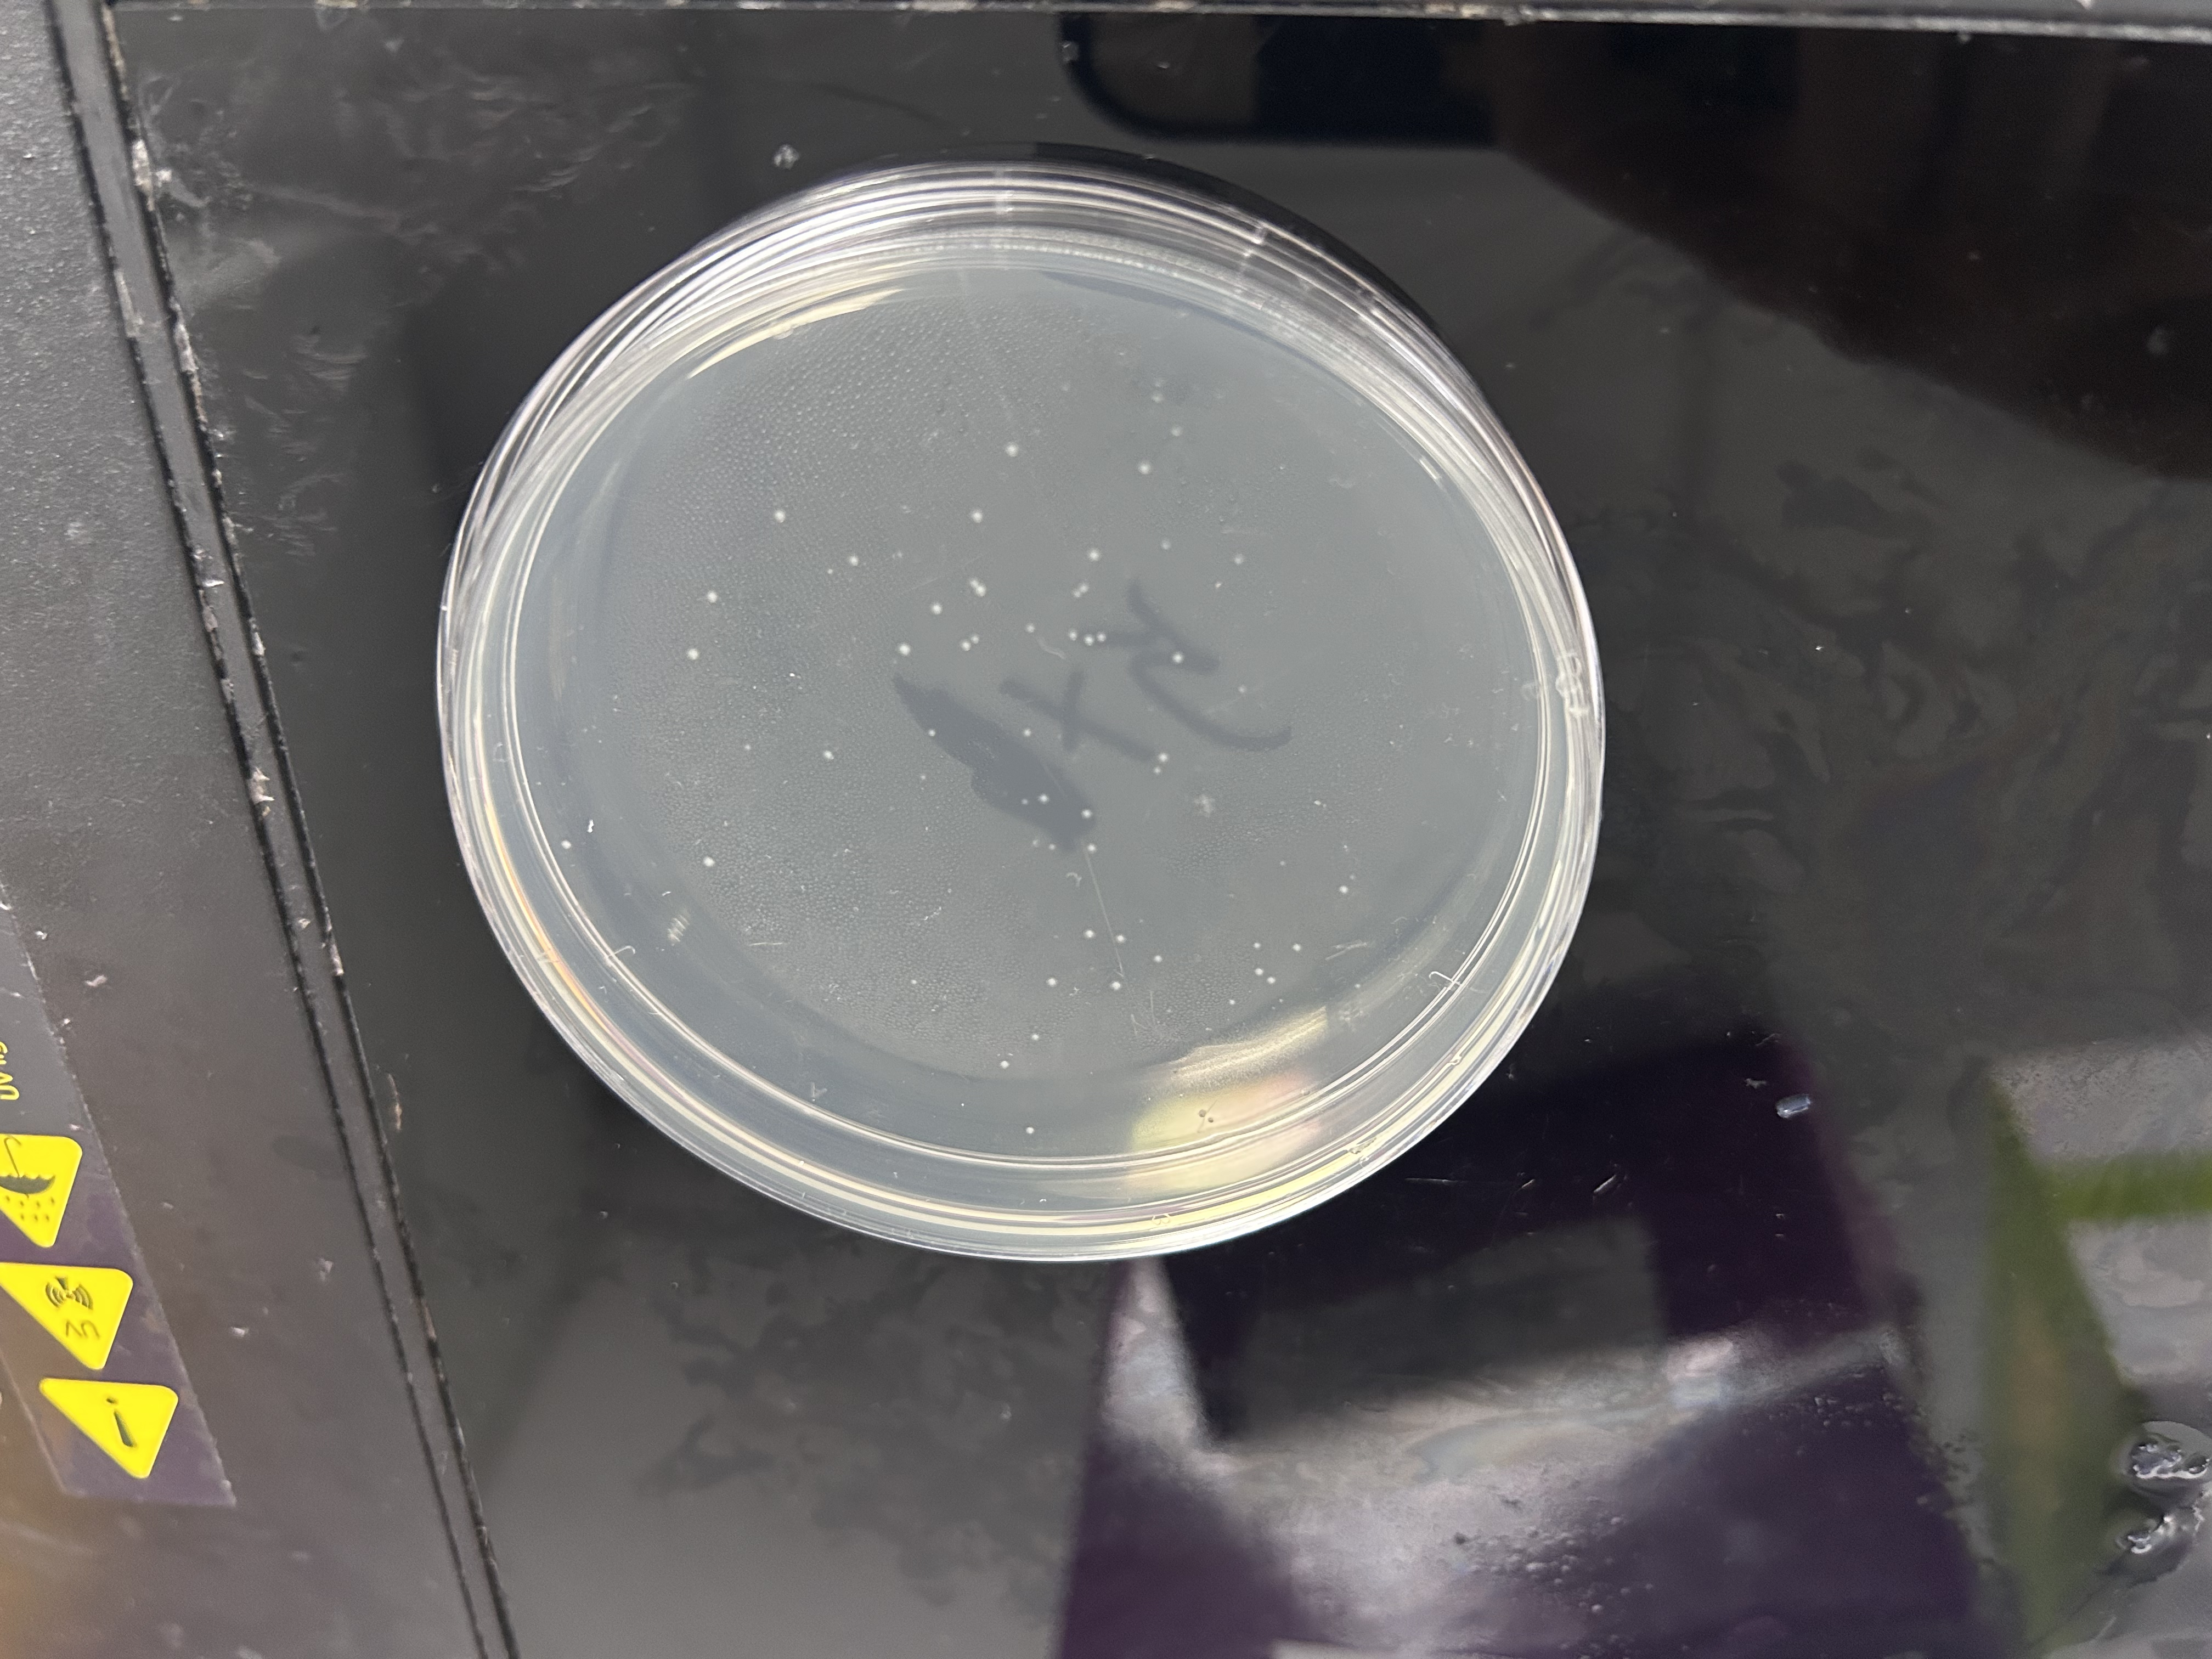
\includegraphics[width=0.3\linewidth]{../Figures/1-5.jpg}}
    \subfigure[(3,5)]{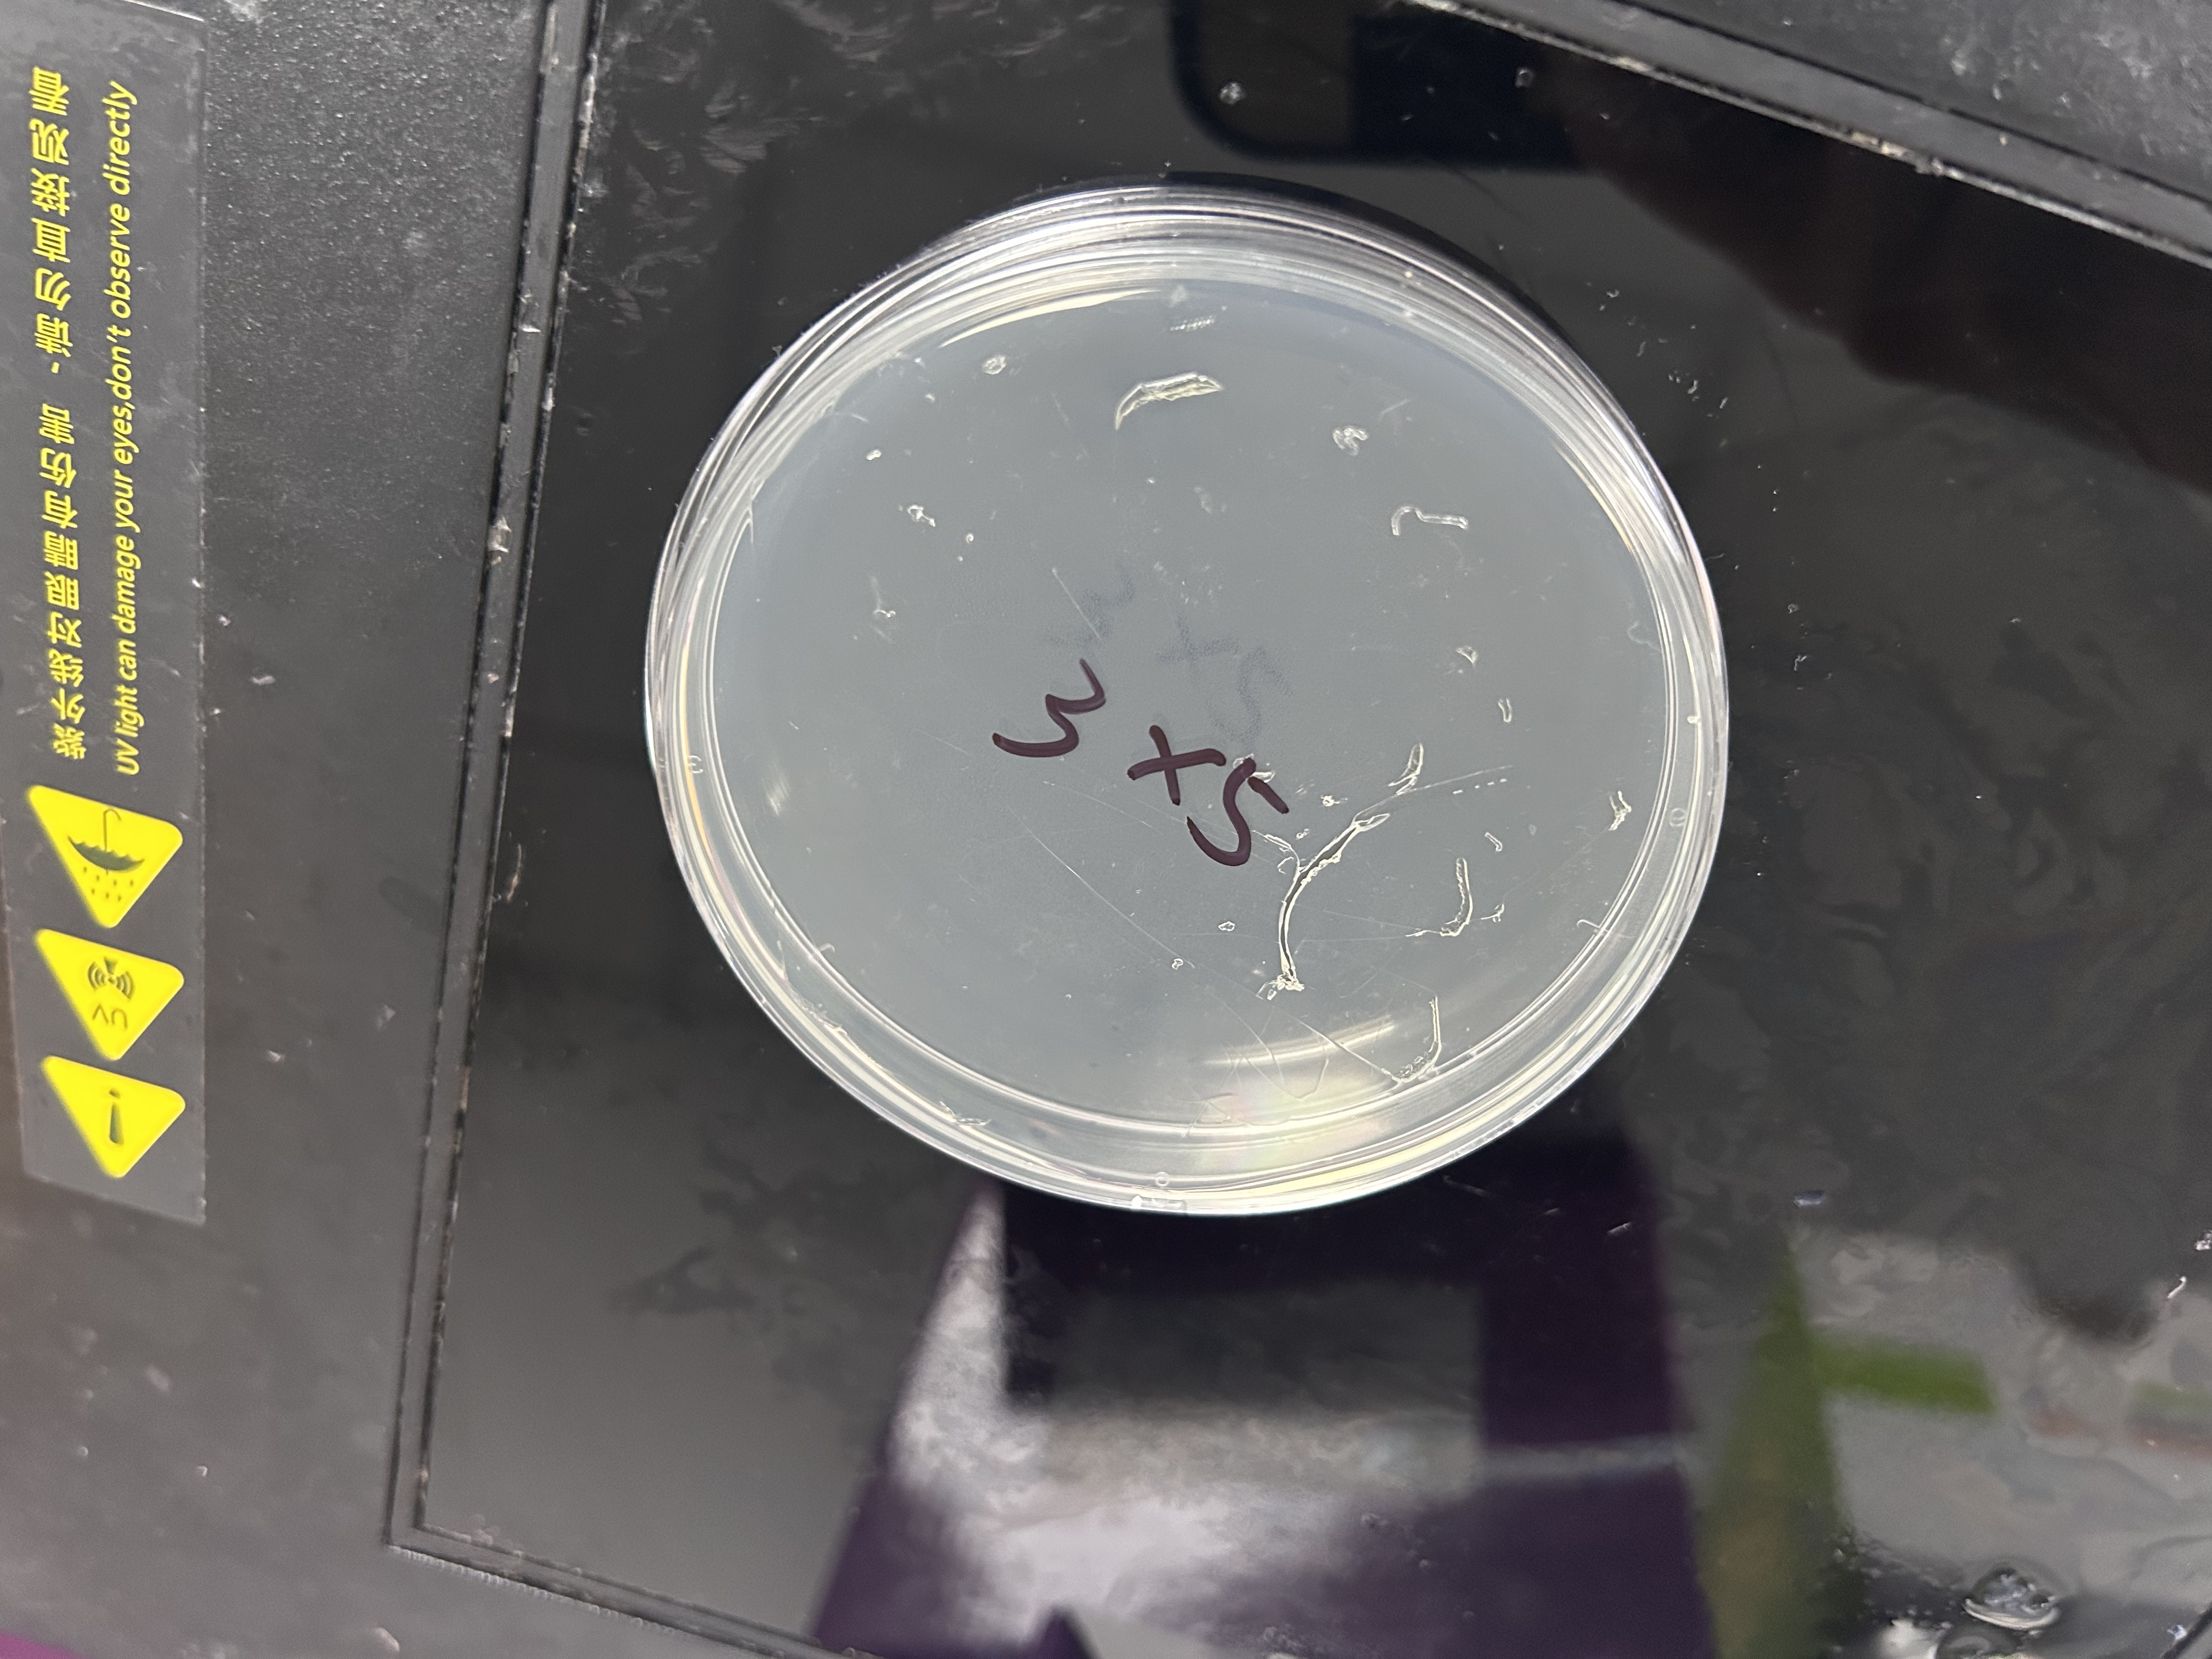
\includegraphics[width=0.3\linewidth]{../Figures/3-5.jpg}}
    \subfigure[(4,5)]{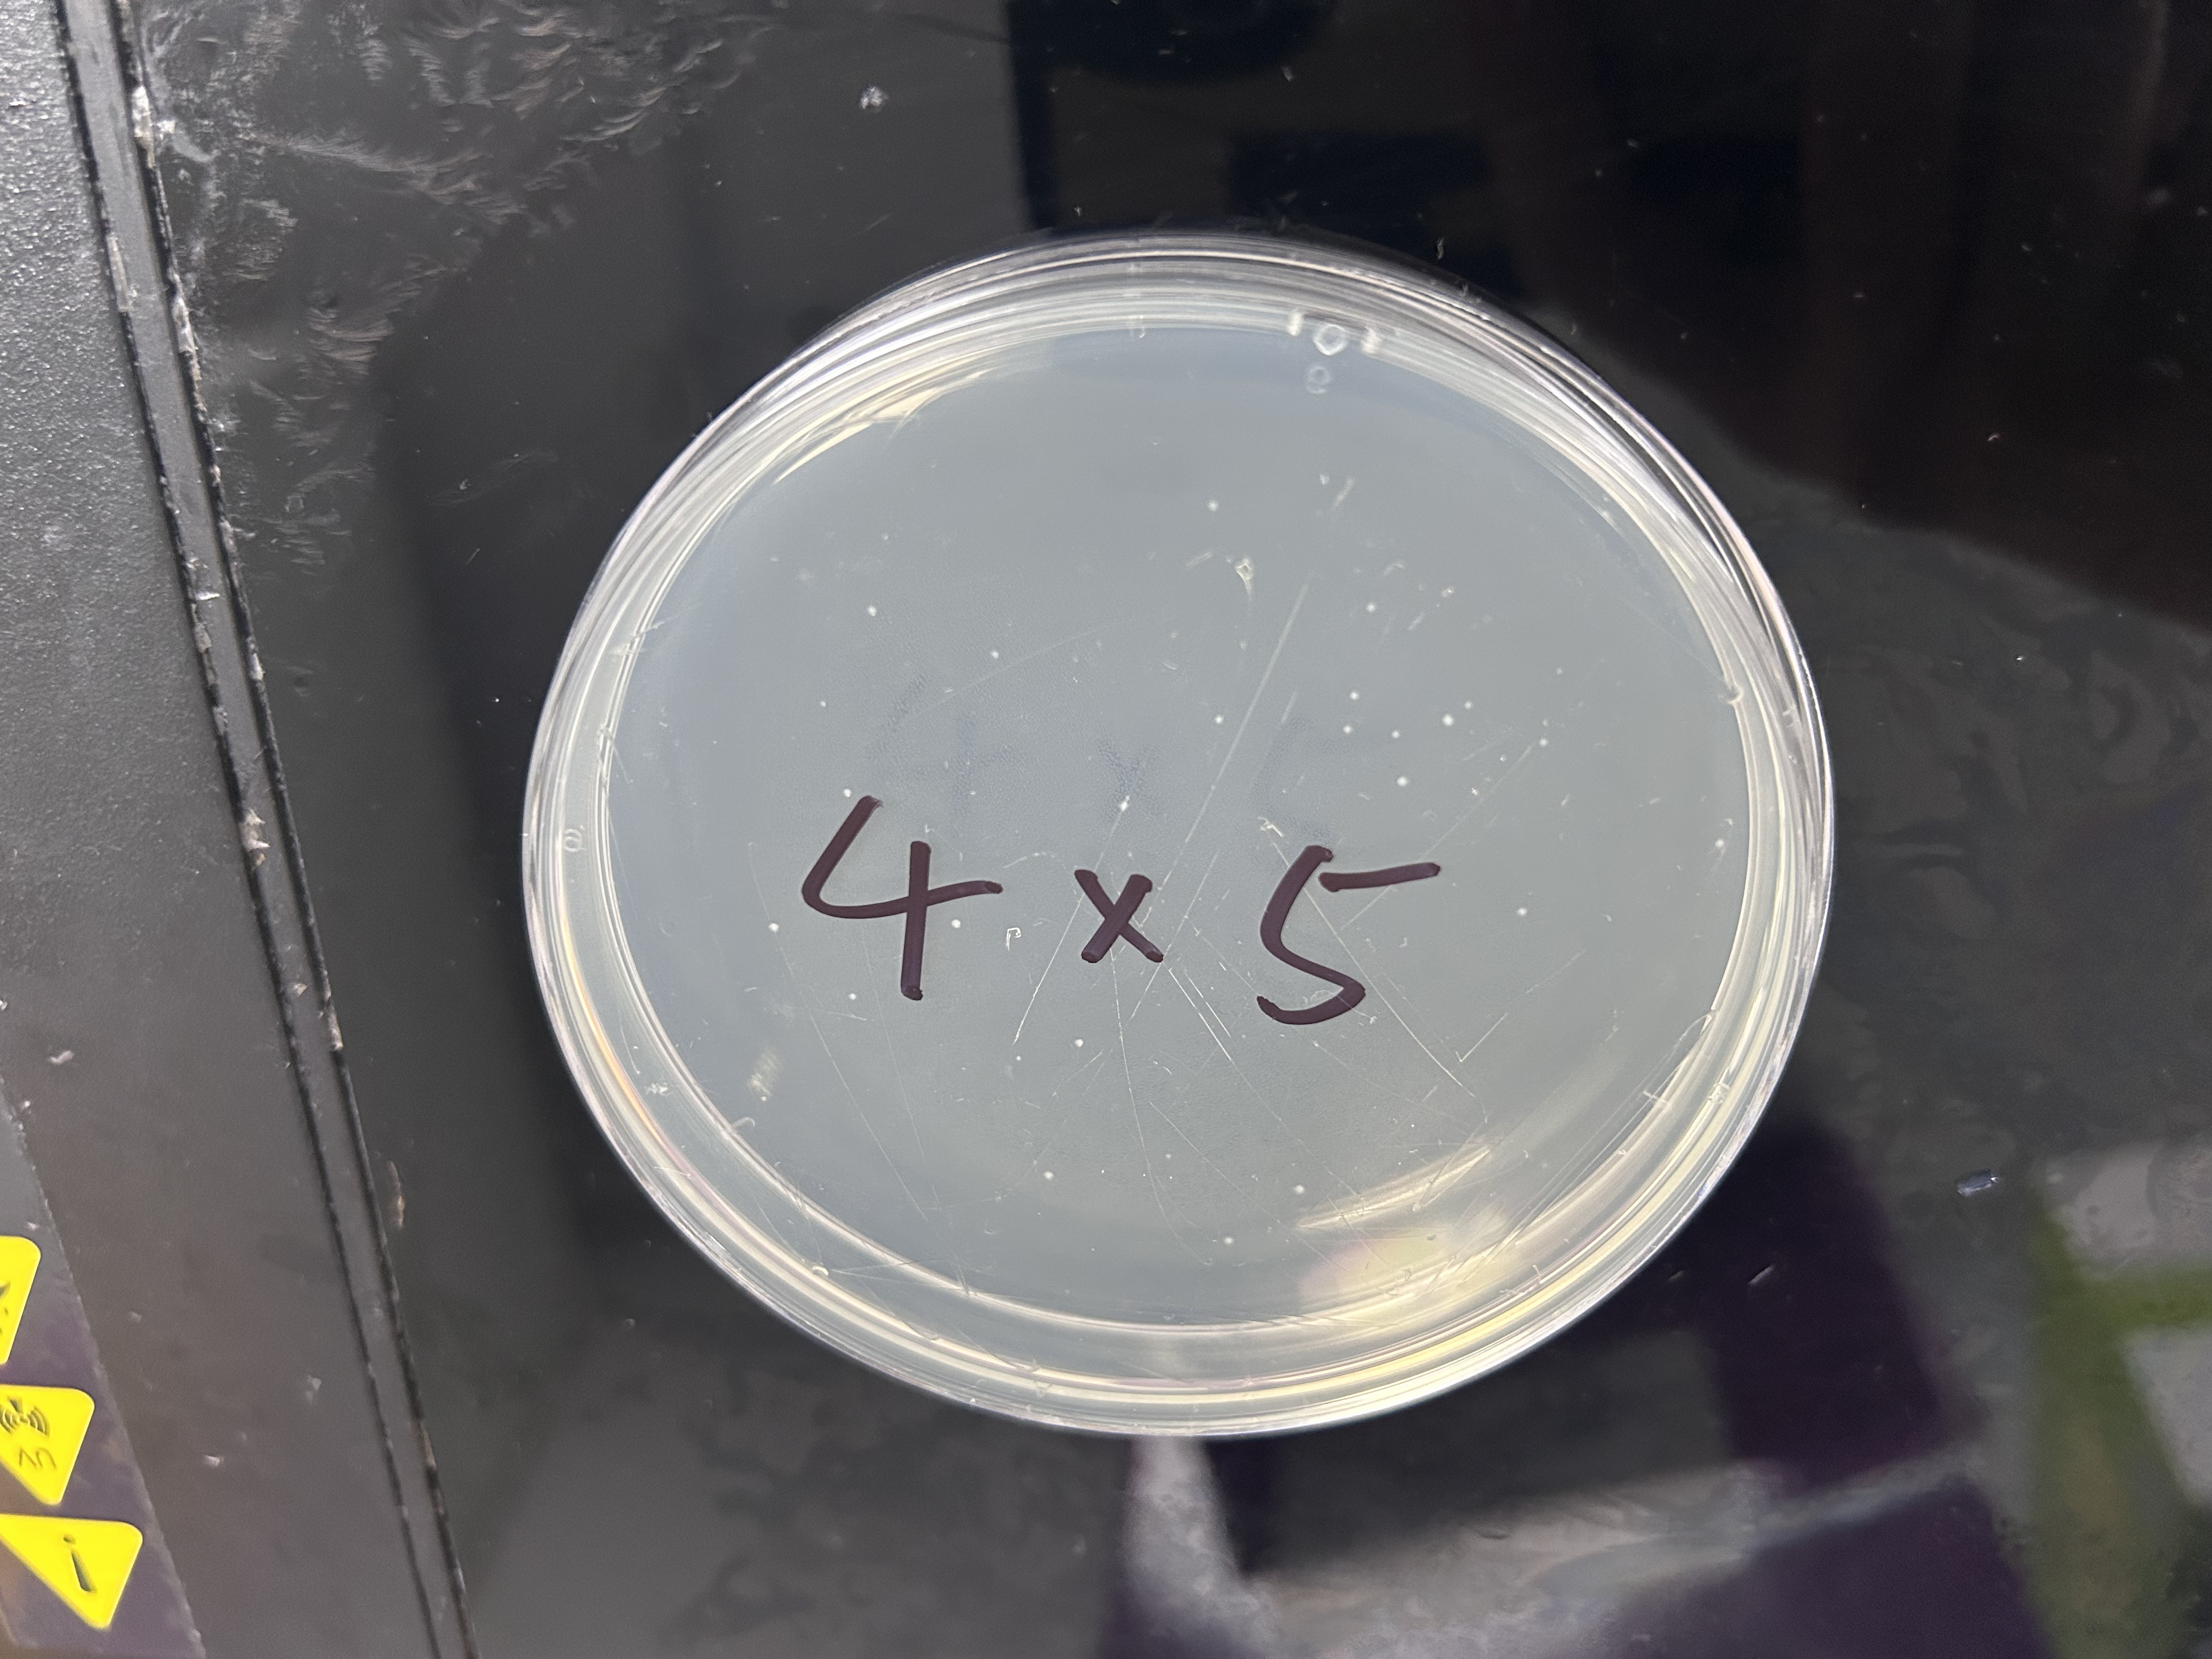
\includegraphics[width=0.3\linewidth]{../Figures/4-5.jpg}}
    \subfigure[(1,6)]{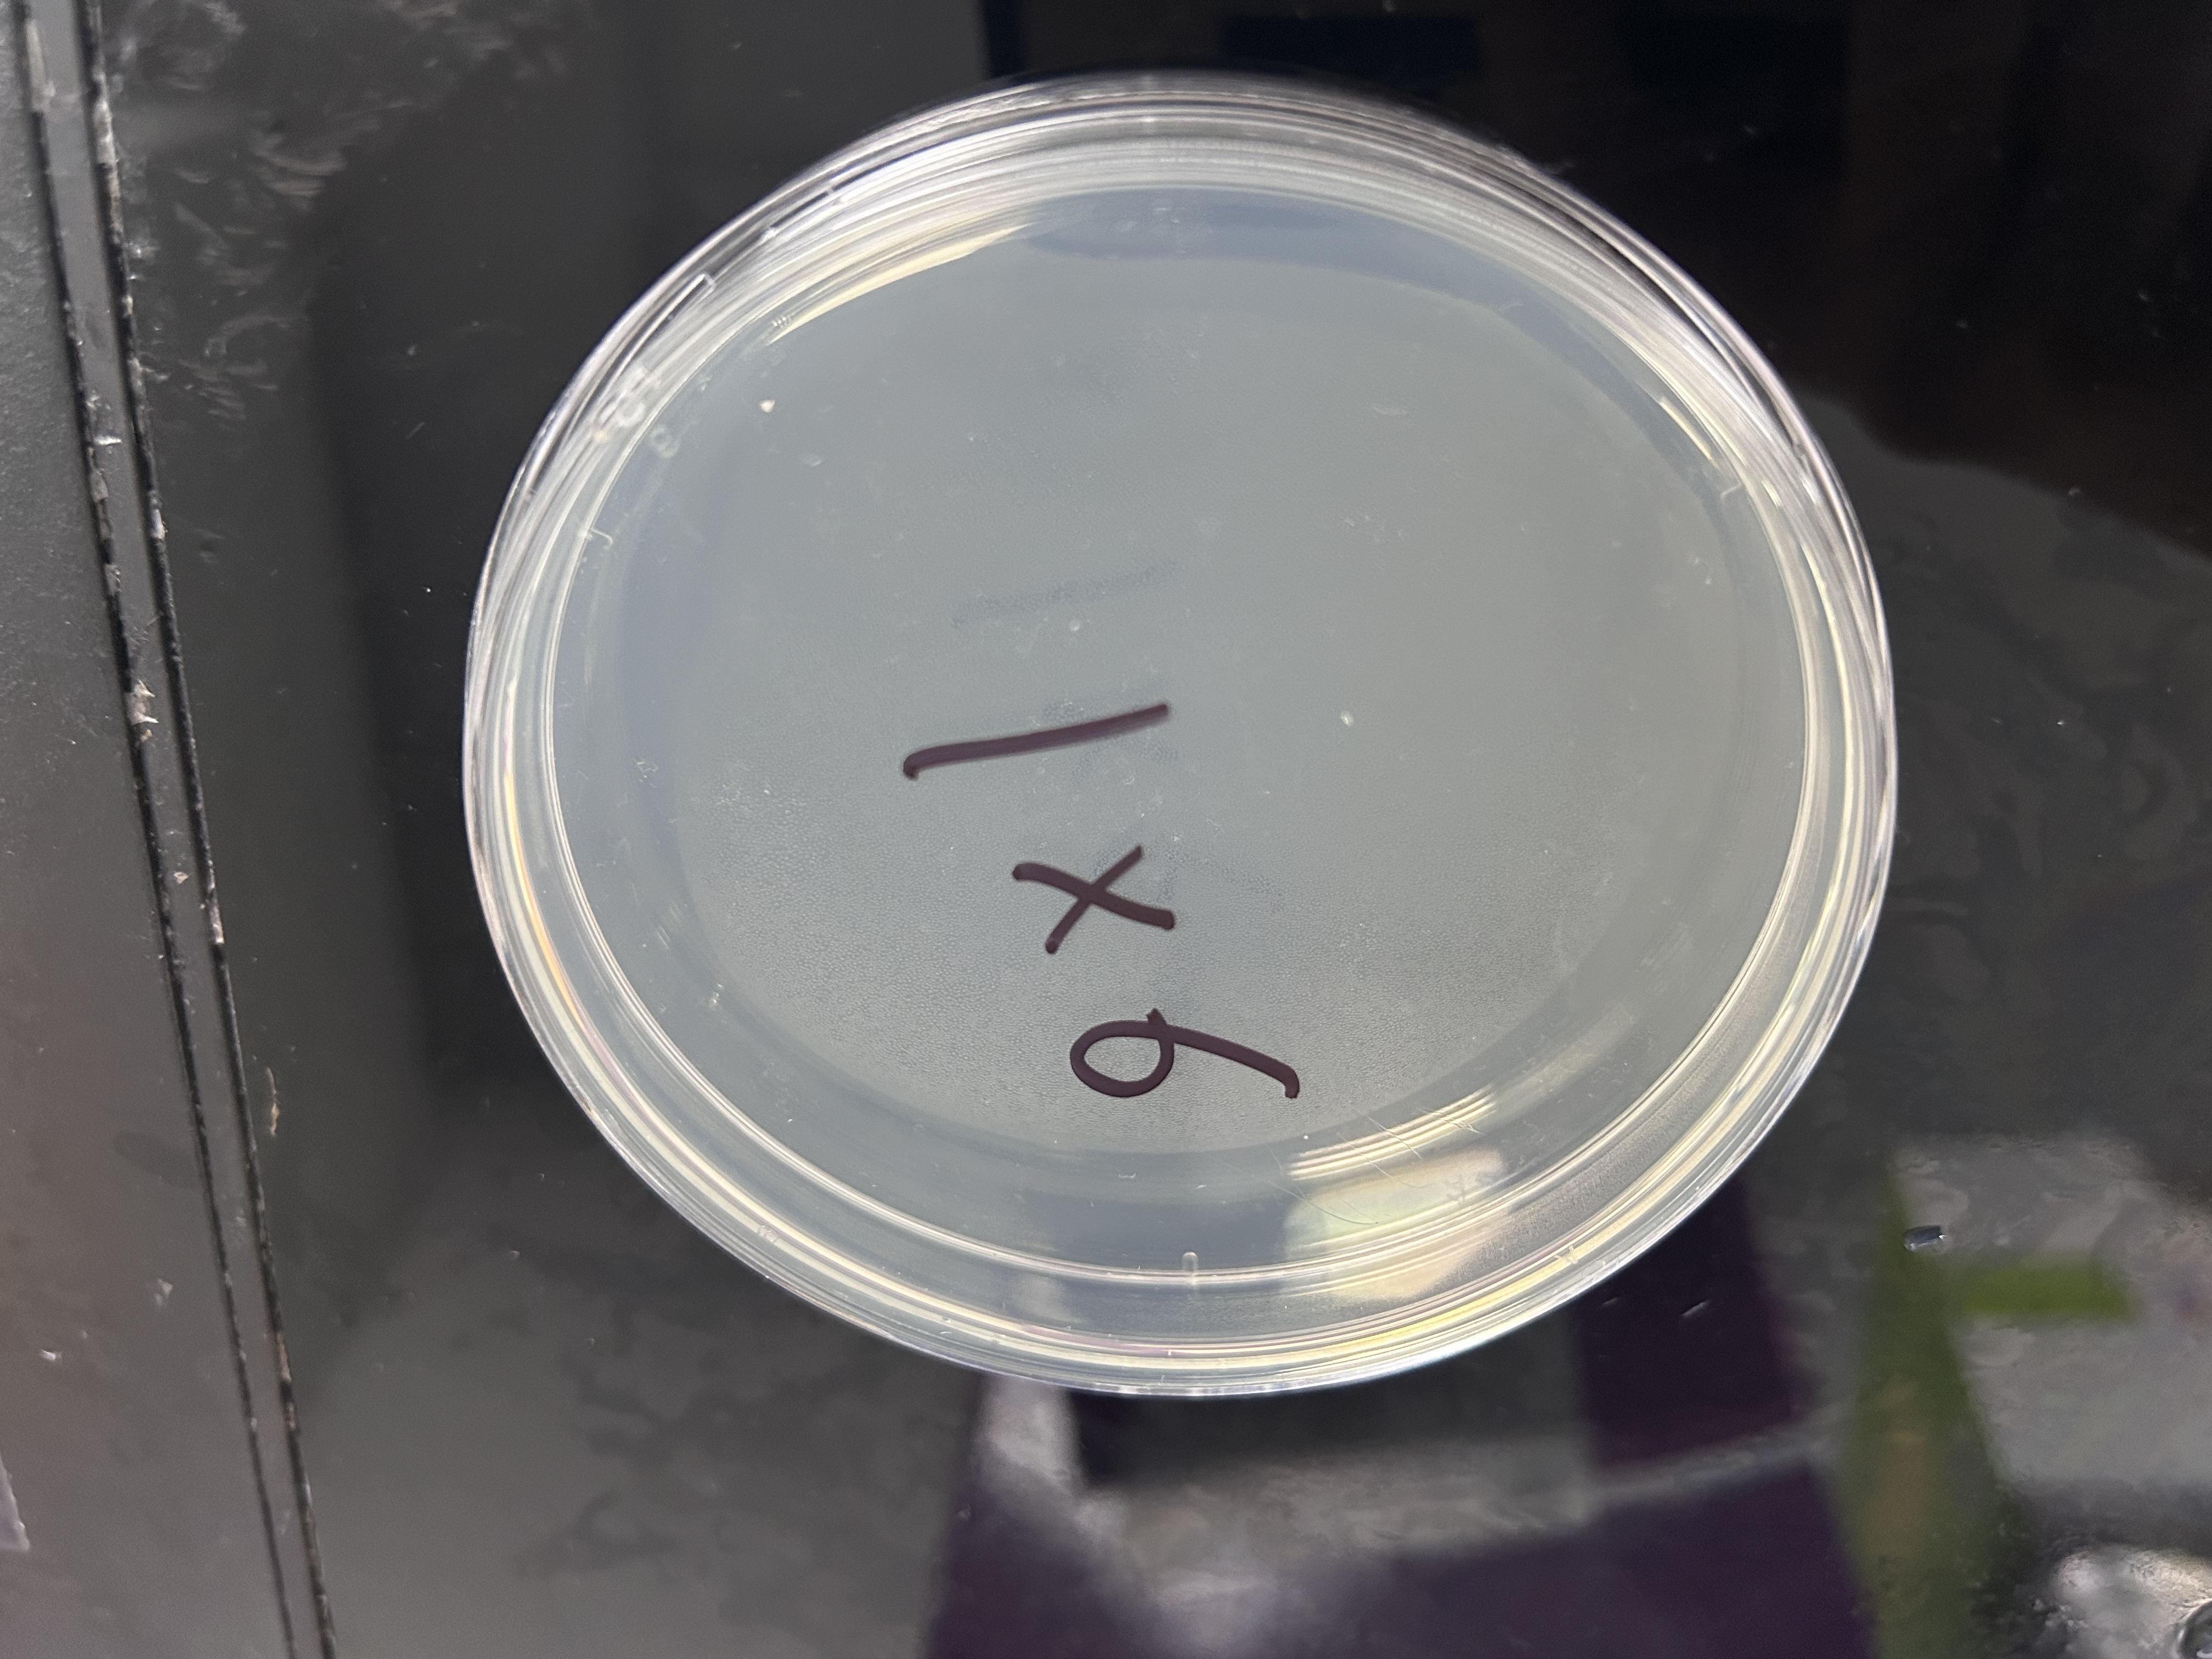
\includegraphics[width=0.3\linewidth]{../Figures/1-6.jpg}}
    \subfigure[(3,6)]{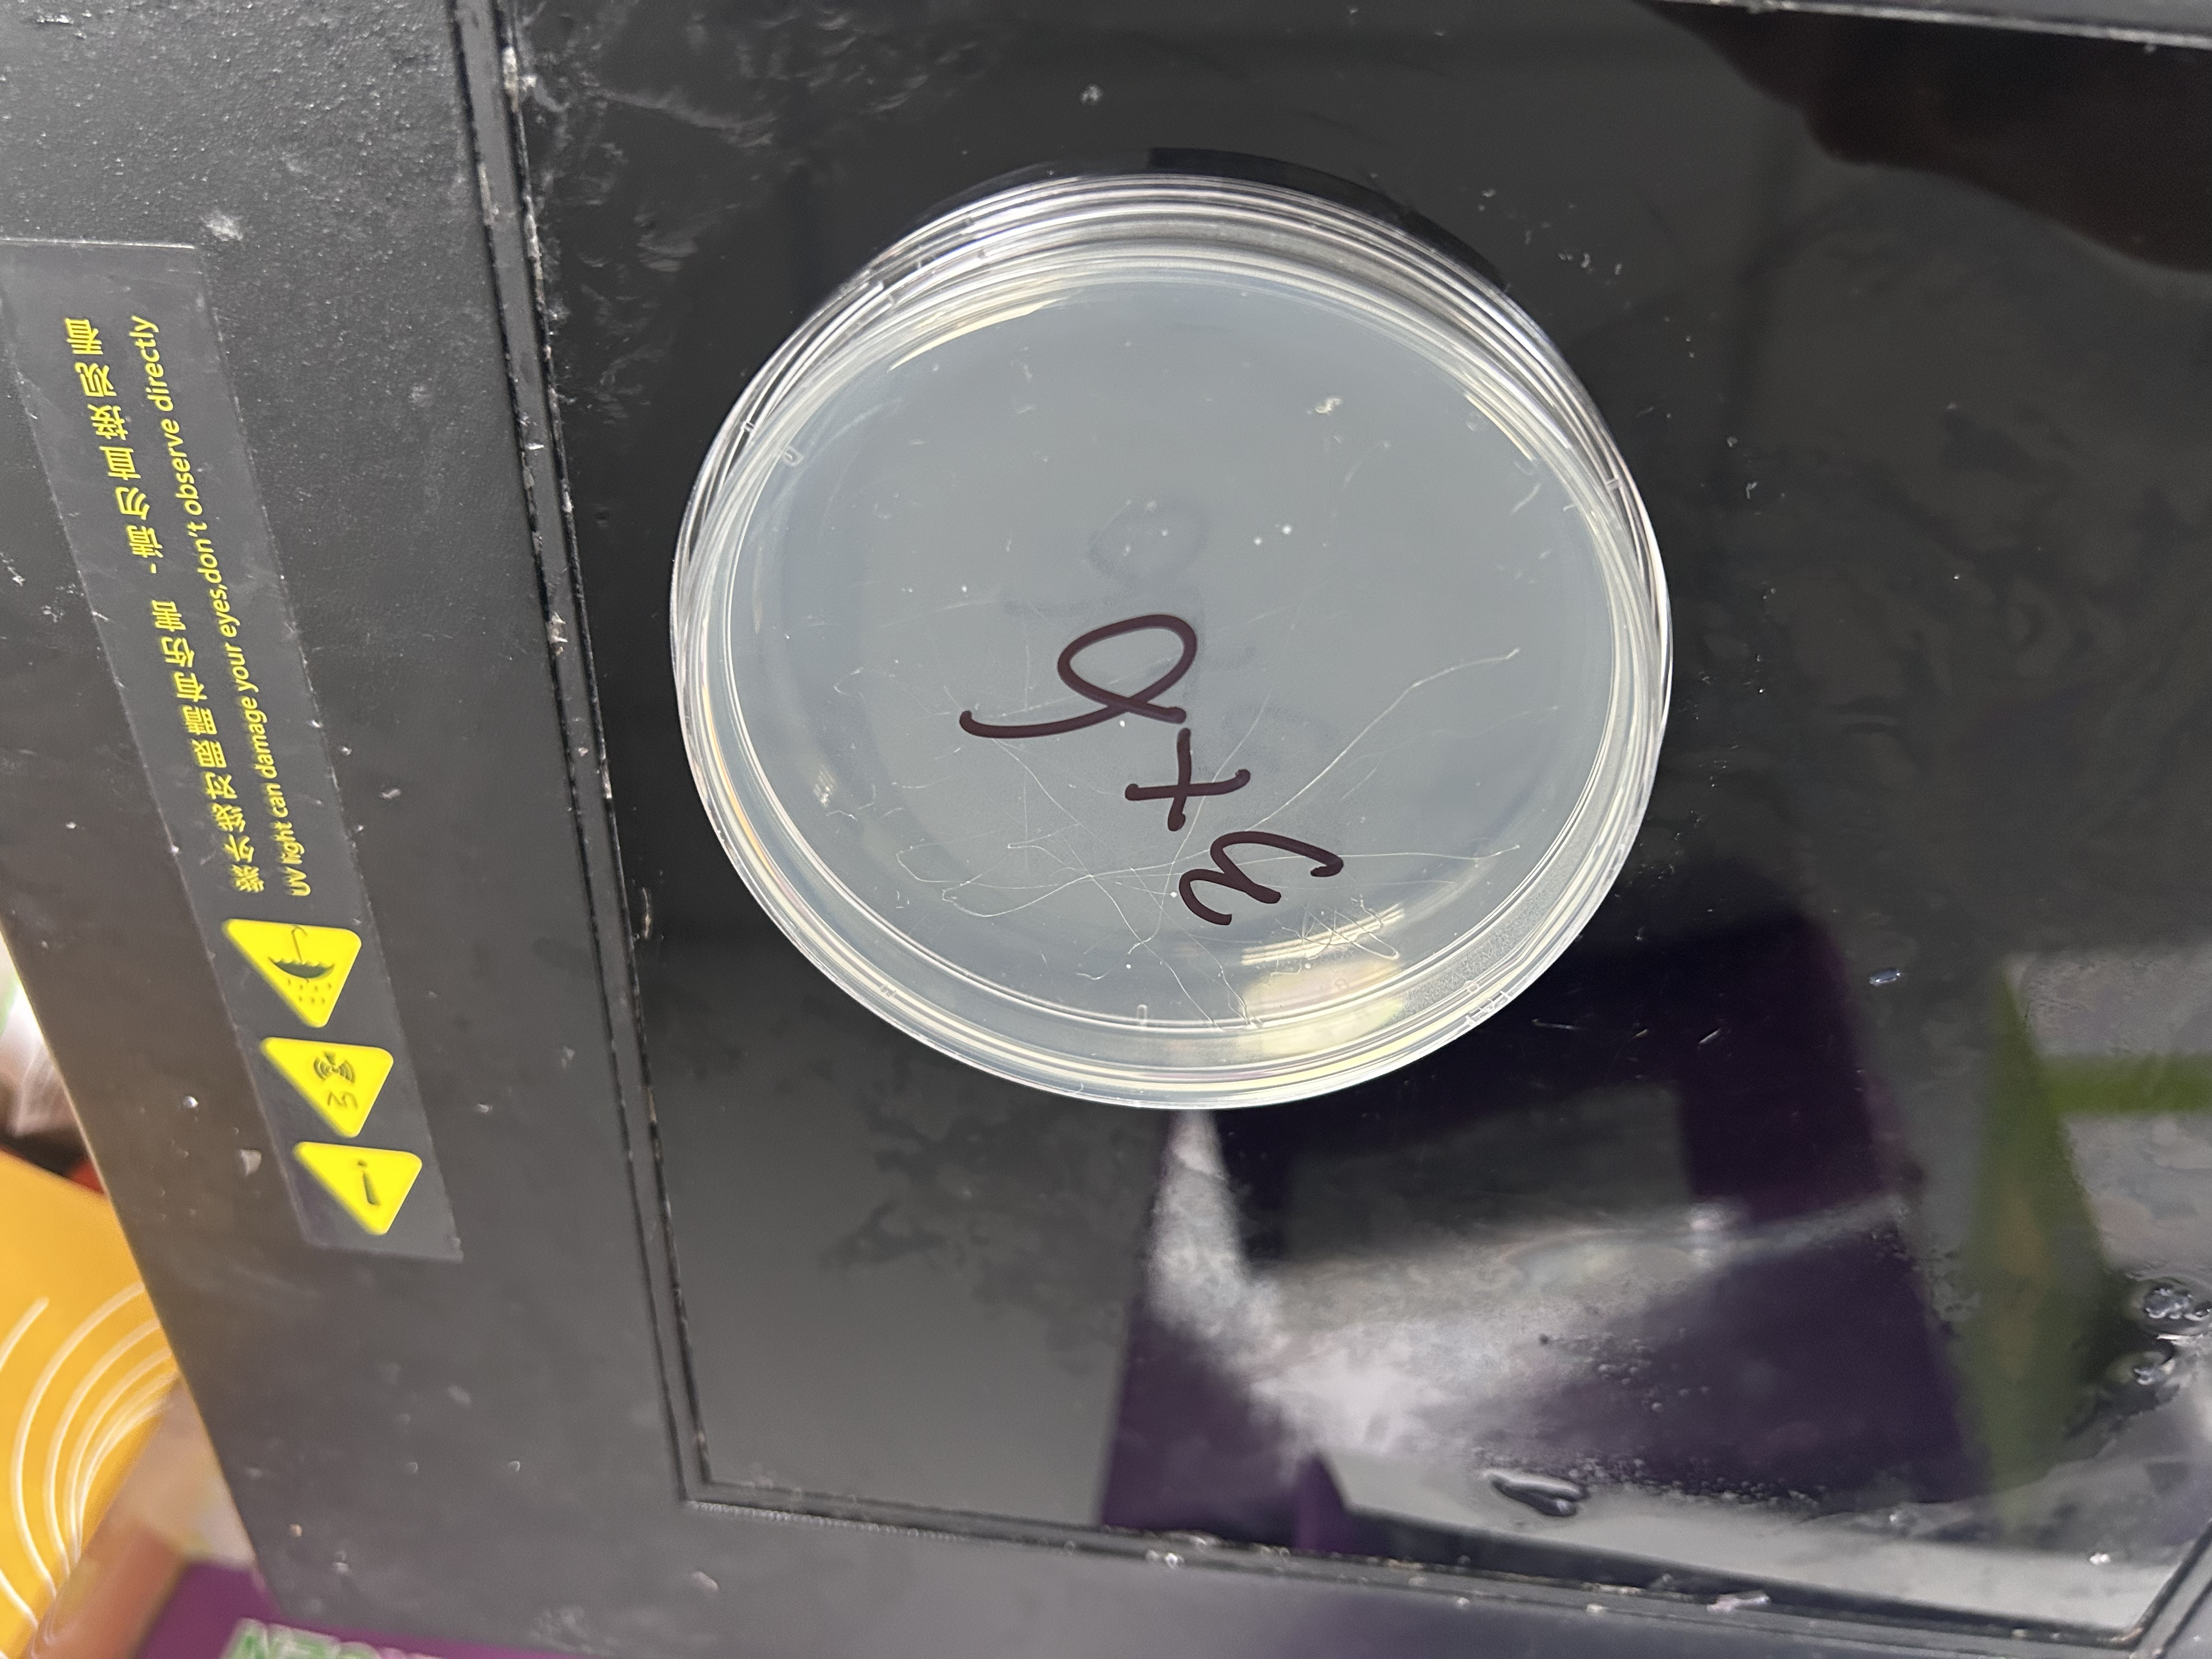
\includegraphics[width=0.3\linewidth]{../Figures/3-6.jpg}}
    \subfigure[(4,6)]{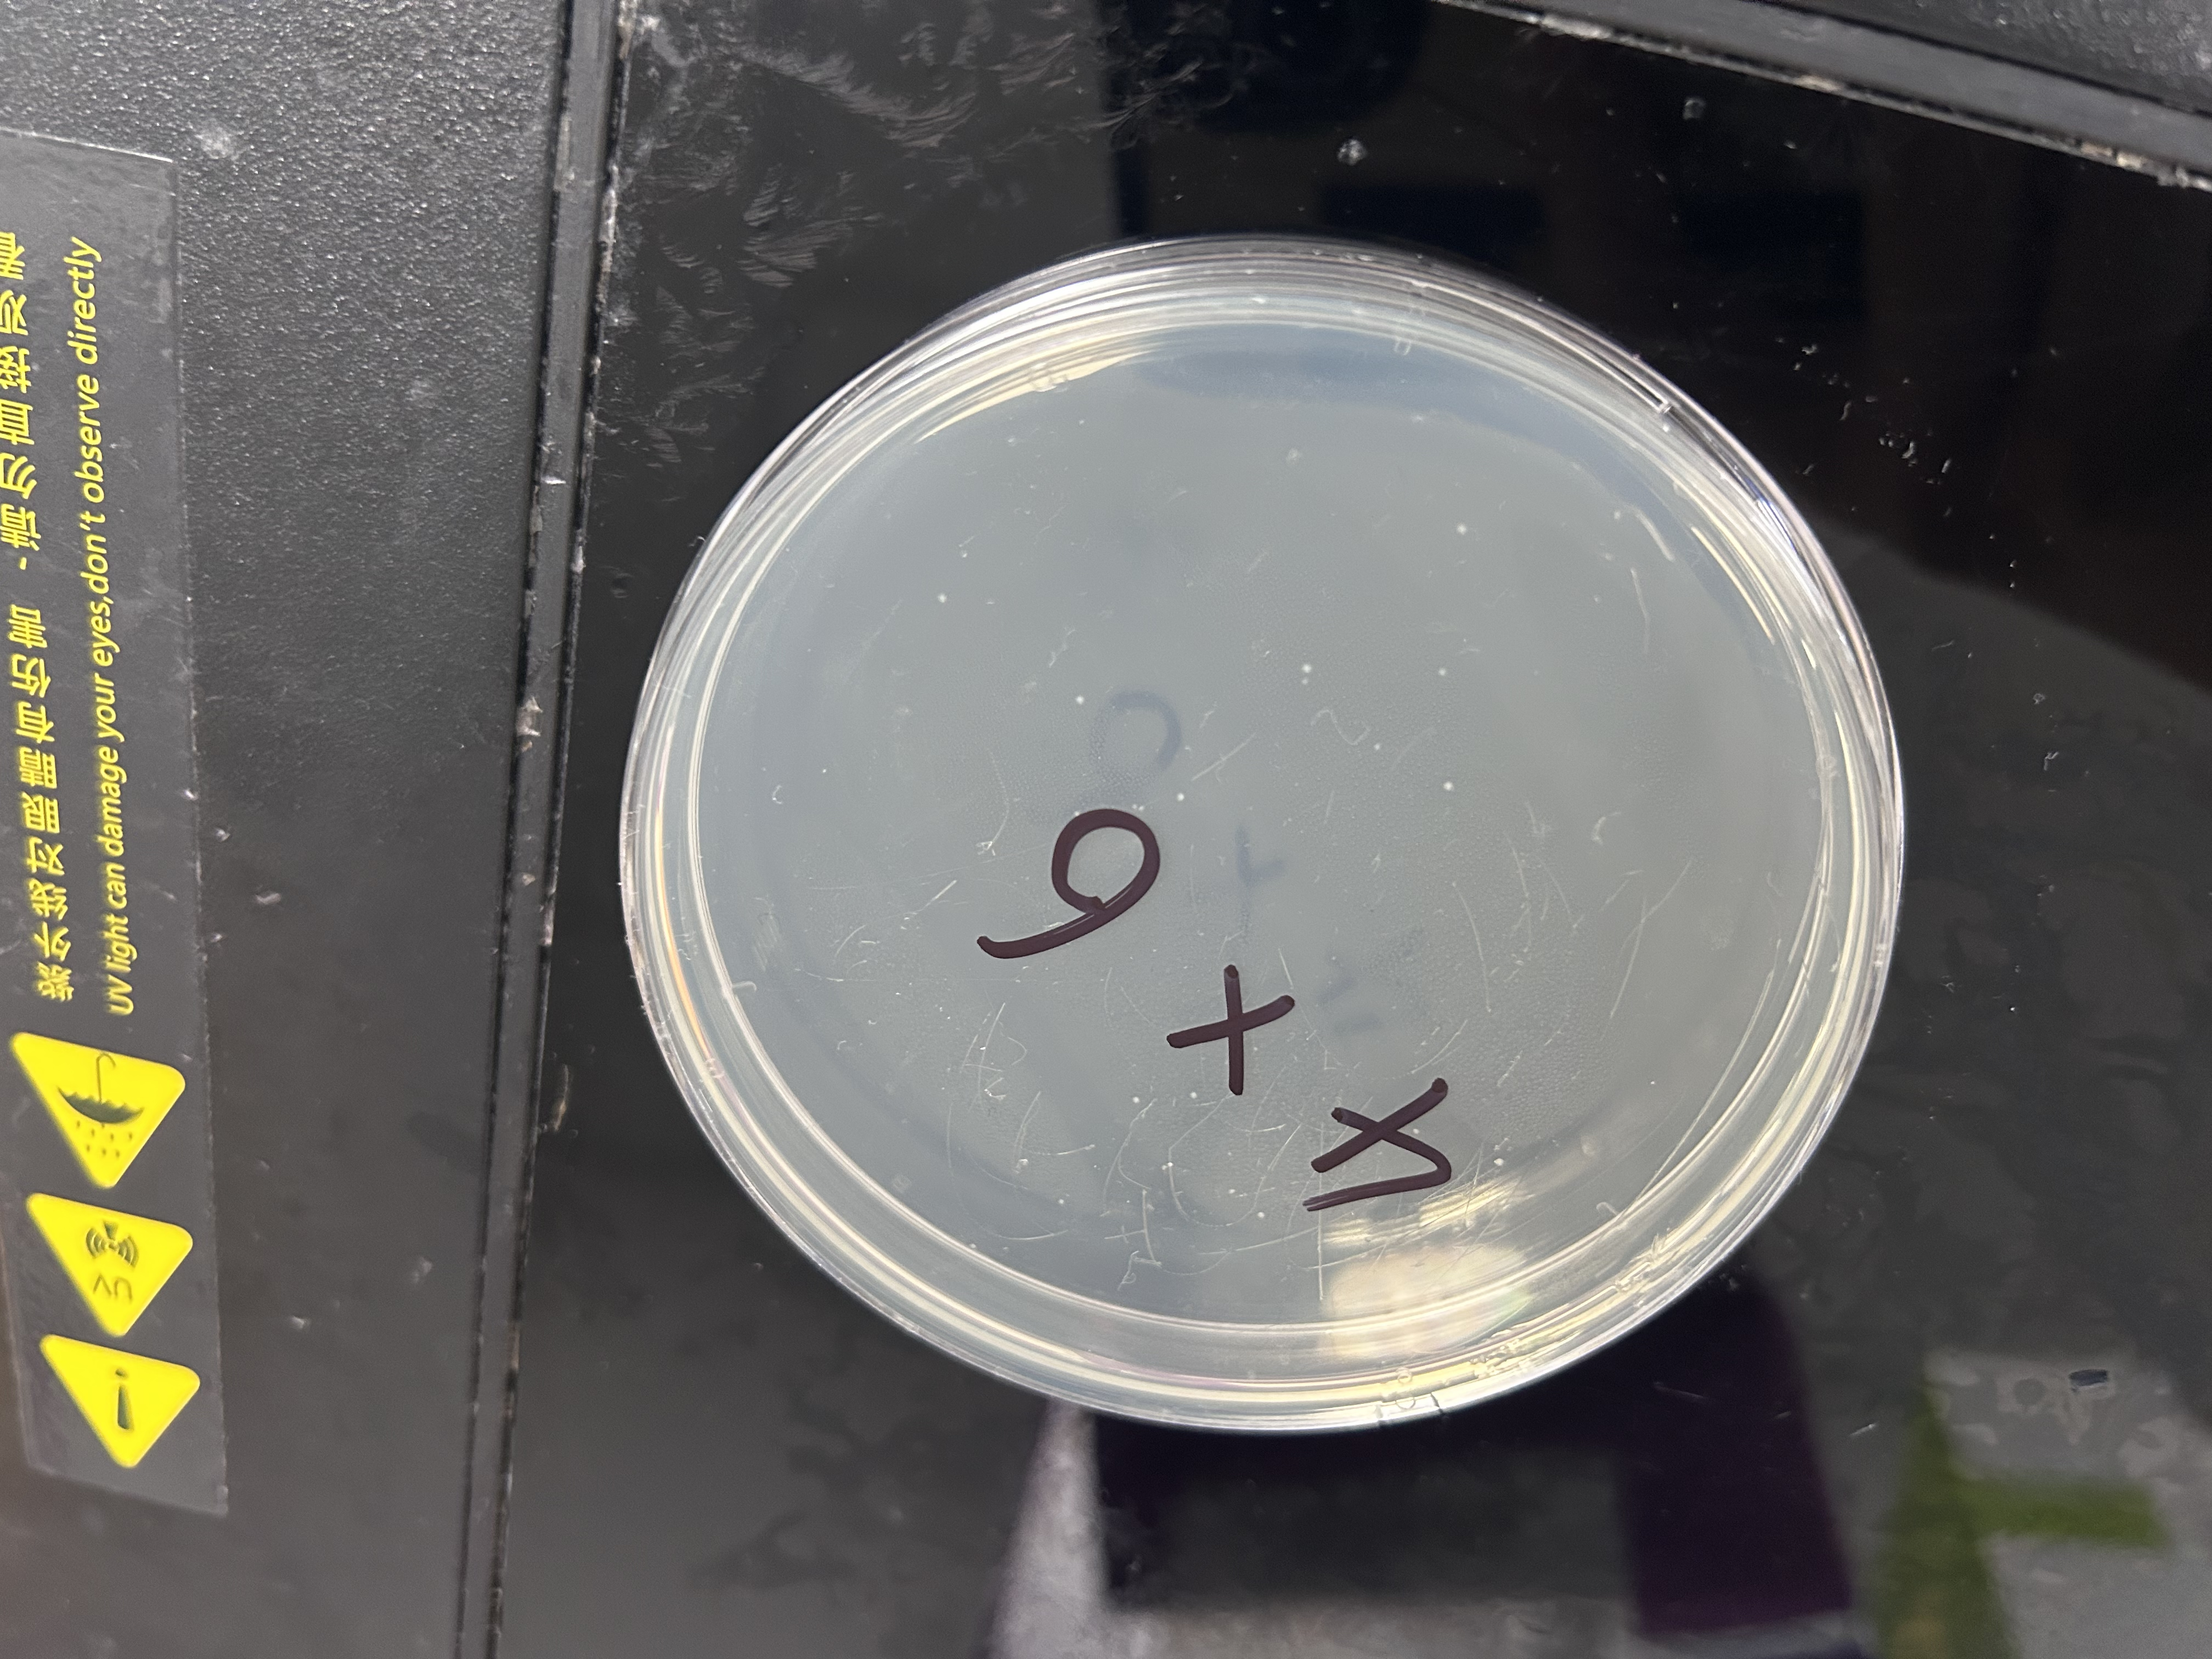
\includegraphics[width=0.3\linewidth]{../Figures/4-6.jpg}}
    
    \caption{Results of Transformation}
    \label{Results of Transformation}
\end{figure}


\bibliographystyle{plain}
\bibliography{references}
\end{document}